%\usepackage{amssymb}
%\usepackage{amsmath}
\subsubsection{Actividad 3 lab 2}
%*********************
\begin{frame}{}

\pgfdeclareimage[width=\paperwidth,height=\paperheight]{bg}{imagenes/fondo_seccion}
\setbeamertemplate{background}{\pgfuseimage{bg}}

\definecolor{greenU}{RGB}{212,202,72}
\setbeamercolor{block body}{fg=Black,bg=greenU}
\begin{block}{}
	\centering
	\vspace{1mm}
	\large{\textit{solucion lab 2 actividad 3}}
	\vspace{1mm}
\end{block}
\end{frame}
%*********************


\begin{frame}{Respuesta Actividad 3 lab 2}
\begin{figure}[H]
\begin{flushleft}
\textbf{Curvas de Lissajous} Las curvas de Lissajous fueron descubiertas por el físico francés Julio Antoine Lissajous 
(1822 a 1880). Fueron utilizadas para determinar las frecuencias de sonidos o de señales de radio, ademas permiten el 
estudio de los movimientos vibratorios y, particularmente, la comparación de los sonidos dados por dos instrumentos. 
\end{flushleft}
\end{figure}
\end{frame}
%--------------------------------
\begin{frame}{Respuesta Actividad 3 lab 2}
\begin{figure}[H]
	\vspace{-3mm}
	\centering
	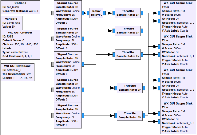
\includegraphics[width=0.9\textwidth]{soluciones/actividad-2-2/pdf/Rlab2_3_1.pdf}
\end{figure}
\end{frame}

%--------------------------------
\begin{frame}{Respuesta Actividad 3 lab 2}
\begin{figure}[H]
	\vspace{-3mm}
	\centering
	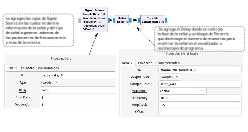
\includegraphics[width=0.9\textwidth]{soluciones/actividad-2-2/pdf/Rlab2_3_2.pdf}
\end{figure}
\end{frame}

%--------------------------------
\begin{frame}{Respuesta Actividad 3 lab 2}
\begin{figure}[H]
	\vspace{-3mm}
	\centering
	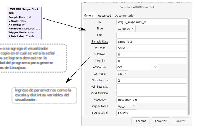
\includegraphics[width=0.9\textwidth]{soluciones/actividad-2-2/pdf/Rlab2_3_3.pdf}
\end{figure}
\end{frame}
%--------------------------------

\begin{frame}{Respuesta Actividad 3 lab 2}
\begin{figure}[H]
	\vspace{-3mm}
	\centering
	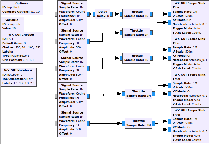
\includegraphics[width=0.9\textwidth]{soluciones/actividad-2-2/pdf/Rlab2_3_4.pdf}
\end{figure}
\end{frame}

%--------------------------------

\begin{frame}{Respuesta Actividad 3 lab 2}
\begin{figure}[H]
	\vspace{-3mm}
	\centering
	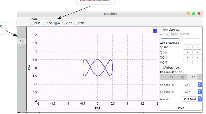
\includegraphics[width=1.1\textwidth]{soluciones/actividad-2-2/pdf/Rlab2_3_5.pdf}
\end{figure}
\end{frame}